\documentclass[TFG.tex]{subfiles}

\begin{document}


%\hyphenation{equi-va-len-cia}\hyphenation{pro-pie-dad}\hyphenation{res-pec-ti-va-men-te}\hyphenation{sub-es-pa-cio}
\chapter{Representaciones lineales}

La existencia (o no existencia) de representaciones lineales fieles de los grupos de trenzas fue uno de los mayores problemas del campo. Este problema fue por primera vez resuelto por Bigelow \cite{Bigelow} y Krammer \cite{Krammer} en el año 2000, mediante la conocida como \emph{representación LKB}. Además de esta representación existen otras, como la representación de Burau, con la cual empezaremos este capítulo.

\section{Representación de Burau}

\subsection{Definición a partir de espacios recubridores}

Consideremos el disco agujereado $n$ veces $\D_n$ con un punto base $d_0\in\D_n$. 
\begin{defi}
Para cada lazo $\alpha$ basado en $d_0$ denominamos \emph{índice total}  a la suma de los índices (número de vueltas) de $\alpha$ con respecto a cada agujero y lo denotamos $\phi\alpha$. Esto es, si un $\alpha$ está representado en $F_n$ por $\prod_{i=1}^n x_i^{m_i}$, entonces 
\[
\phi\alpha=\sum_{i=1}^nm_i.
\]
\end{defi}

Se observa que $\phi$ es un homomorfismo de grupos $\phi:\pi_1(\D_n)\to\Z$ al ser el índice total un invariante homotópico. Sea $\tilde{\D}_n$ el espacio recubridor correspondiente a $\ker\phi$. Vamos a describir geométricamente este espacio recubridor (ver Figura \ref{recubrimiento}). 

%si es invariante homotópico también lo será por homeomorfismo

Para visualizarlo mejor, vamos a agrandar los agujeros de modo que se conviertan en bolas abiertas y llamamos a este nuevo espacio $X$. Dibujamos segmentos $A_1,\dots, A_n$ desde el centro de las bolas hasta el borde del disco. Cortamos $X$ a lo largo de estos segmentos, de modo que obtenemos dos copias disjuntas $A_i^+$ y $A_i^-$ de cada $A_i$. Llamamos a este espacio $X^*$. Sean $h_i:A_i^+\to A_i^-$ homeomorfismos y tomamos una cantidad numerable de copias $X^*_j$ de $X^*$. Para cada $j$ sea $g_j:X^*_j\to X^*$ un homeomorfismo. El espacio $\tilde{X}$ se define como la unión disjunta de los $X^*_j$ identificando $A_i^+\subseteq X^*_j$ con $A_i^-\subseteq X^*_{j+1}$ mediante $g_{j+1}^{-1}h_ig_j$.

%Se idenfitica A_i^+ con la imagen mediante la aplicación esa

\begin{figure}[h!]
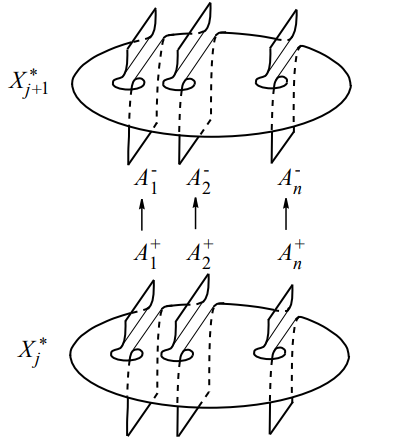
\includegraphics[scale=0.6]{Imagenes/recubrimiento}
\caption{Dos hojas del espacio recubridor $\tilde{X}$.}\label{recubrimiento}
\end{figure}

El hecho de que este sea el recubrimiento correspondiente a $\ker\phi$ se debe a que, fijada una preimagen $\tilde{d}_0\in\tilde{X}$ preimagen de $d_0$, un lazo en $d_0$ se levanta a un lazo en $\tilde{d}_0$ si y solo si su índice total es nulo, pues para cada vuelta positiva sube un nivel en el recubrimiento y para cada vuelta negativa lo baja, así que para acabar de nuevo en $\tilde{d}_0$ deberá subir tantas veces como baja, es decir, que el número total de vueltas sea nulo.

Hay una acción natural de $\Z$ en $\tilde{X}$ dada por $X^*_j\ni x\mapsto g_{j+n}^{-1}g_jx$ para cada $n\in\Z$. Esta acción se puede interpretar como cambiar el punto $x$ de nivel. Además, la acción es claramente libre y el espacio de órbitas $\tilde{X}/\Z$ es $X$, por lo que el espacio recubridor es regular.


¿PODRÍA DEFINIRLO ASÍ QUE ES MÁS SENCILLO EN LUGAR DE DEFINIRLO A PARTIR DE LAS TRANSFORMACIONES DE DECK QUE EMPIEZA COGIENDO AUTOMORFISMOS SOBRE LAS FIBRAS?


Vamos a ver cómo definir la representación de Burau. Sea $\beta\in B_n$ inducida por un automorfismo $h$ de $\D_n$ fijando el borde, lo cual vamos a denotarlo $\beta=h_*$. Entonces, para cualquier lazo $\gamma$ en $\D_n$ se tiene que $\phi(h\gamma)=\gamma$, de modo que $h$ se levanta a un automorfismo $\tilde{h}$ de $\tilde{\D}_n$ que fija el borde. Pasando a la homología, esto nos da un automorfismo de $H_1(\tilde{\D}_n)$. Si $h'$ es cualquier otro automorfismo con $h'_*=\beta$, entonces $h_*^{-1}h'_*=1$, así que como la aplicación inducida por el recubrimiento $\pi_1(\tilde{\D}_n)\to\pi_1(\D_n)$ es inyectiva \cite{Hatcher} tenemos que $\tilde{h}_*^{-1}\tilde{h}'_*=1$ como aplicación en $\pi_1(\tilde{\D}_n)$. Pasando a homología, esto nos da $\tilde{h}'_*-\tilde{h}_*=1$ como aplicación en $H_1(\tilde{\D}_n)$. 

¿EL SEGUNDO PASO A HOMOLOGÍA SE HACE ABELIANIZANDO CON HUREWICZ?

AQUÍ TENGO UNA PREGUNTA COMENTADA EN EL TEX
%¿Se puede levantar siempre el automorfismo? Supongo que sí, porque p:X->Dn, h:Dn->Dn, entonces cojo para cada fibra p^{-1}hp: X -> X. Como en los segmentos coincide para cada fibra, se extiende a todo X. 


\begin{defi}
Sea el homomorfismo $\psi_r:B_n\to GL(H_1(\tilde{\D}_n))$ dado por $\psi_r(\beta)=\tilde{h}_*$. Esta aplicación está bien definida por las observaciones anteriores y es lo que se conoce como \emph{representación de Burau reducida} de $B_n$.
\end{defi}

Se llama \emph{reducida} porque existe una representación $n$-dimensional de la cual la forma reducida es un sumando irreducible. Esta mencionada representación $n$-dimensional puede encontrarse en \cite{thesis}. Como veremos con la siguiente proposición, la representación que hemos dado es $n-1$-dimensional.

¿SUMANDO IRREDUCIBLE QUÉ SIGNIFICA? ¿COMO SUMA DIRECTA?

\begin{prop}
$H_1(\tilde{\D}_n)$ es un módulo libre de rango $n-1$ sobre $\Z[t,t^{-1}]$.
\end{prop}
\begin{dem}
\end{dem}


%Lo de que se corresponda al ker es como cuando en Hatcher hace corresponder un espacio recubridor de S1vS1 a cada grupo libre generado con combinaciones de los lazos ab. Como explica Hatcher, se hace cogiendo la imagen del homomorfismo inducido por el recubrimiento en el grupo fundamental del recubrimiento fijando un punto base preimagen del punto base de X. El subgrupo generado por esta imagen en pi(X,x0) es el que se corresponde con el recubrimiento. En este caso, fijada una preimagen de d0, los lazos en d0 son los que tienen total winding number 0 porque cada vez que hacen un giro bajan o suben de nivel, por lo que para volver a d0 tienen que subir lo mismo que bajan

%el homomorfismo inducido por el recubrimiento en los grupos fundamentales es siempre inyectivo (Hatcher)

%Over a commutative ring R, more care is needed: a matrix over R is invertible if and only if its determinant is a unit in R, that is, if its determinant is invertible in R. Therefore, GL(n, R) may be defined as the group of matrices whose determinants are units.
\subsection{Expresión matricial}

\section{Representación LKB}



\section{Solución al problema de la palabra}

\begin{ej}
\end{ej}

\end{document}
%https://arxiv.org/pdf/math/0006202.pdf
%http://ms.mcmaster.ca/~boden/students/Smeltzer-MSc.pdf
%Creo que el de encima y el de debajo son el mismo
%http://www.numdam.org/article/SB_1999-2000__42__389_0.pdf Aquí comenta cuándo la de Burau es fiel y cuándo no y quiénes lo probaron
%La de Krammer sí es faithful siempre
%LKB http://wrap.warwick.ac.uk/90207/1/WRAP_Theses_Coles_2017.pdf PERO ESTAS COSAS SON SOBRE ANILLOS, NO SOBRE CUERPOS, ME ESTÁ RALLANDO

%Este tiene buena pinta http://go.owu.edu/~chjackso/Papers/thesis.pdf